\chapter{Izvođenje i rezultati}
\label{ch:rezultati}

\section{Primjer izvođenja programa}
\label{sec:izvodjenje}

Program se pokreće iz naredbenog retka naredbom \lstinline!./inverseMapping! kao u prikazu koda \ref{code:pokretanje}.
\begin{lstlisting}[label={code:pokretanje}, caption={Pokretanje programa}]
./inverseMapping originalna_slika.jpg transformirana_slika.jpg sirina_transfomirane_slike visina_transformirane_slike
\end{lstlisting}

Nakon toga se prikazuje prozor s originalnom slikom kao na slici \ref{fig:odabirTocaka1} na kojemu korisnik pokazivačem odabere četiri točke koje predstavljaju kutove dijela slike nad kojim je potrebno obaviti inverznu perspektivnu transformaciju, počevši od lijevog gornjeg u smjeru kazaljke na satu (slika \ref{fig:odabirTocaka2}).

\begin{figure}[ht]
\centering

\begin{subfigure}{0.45\textwidth}
\begin{minipage}{0.9\textwidth}
	\centering
	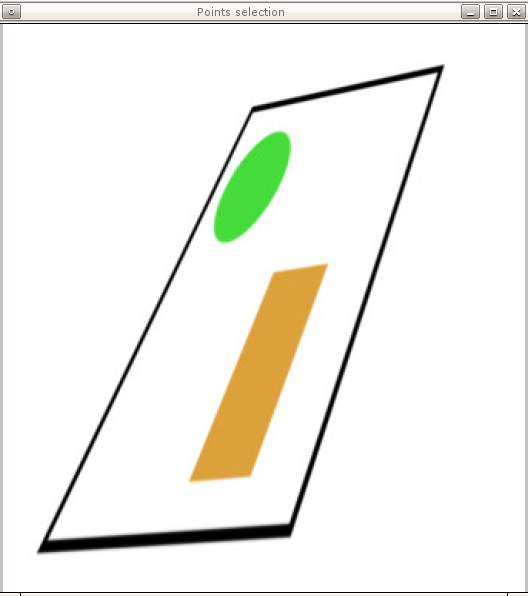
\includegraphics[width=\textwidth]{figures/points_selection.jpg}
	\caption[margin=1cm]{Originalna slika prije odabira točaka}
	\label{fig:odabirTocaka1}
\end{minipage}
\end{subfigure}%
\begin{subfigure}{0.45\textwidth}
\begin{minipage}{0.9\textwidth}
	\centering
	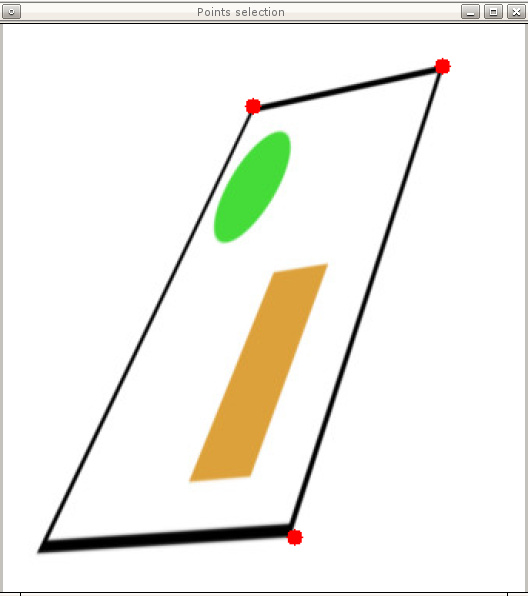
\includegraphics[width=\textwidth]{figures/points_selection_selected.jpg}
	\caption{Originalna slika za vrijeme odabira točaka}
	\label{fig:odabirTocaka2}
\end{minipage}
\end{subfigure}

\caption{Odabir točaka}
\label{fig:odabirTocaka}

\end{figure}

Nakon odabira točaka počinje izračunavanje transformacijske matrice, a nakon toga i sama transformacija slike čiji se napredak može pratiti u konzoli. Kada su svi slikovni elementi transformirani, transformirana se slika sprema u datoteku navedenu u naredbenom retku, a istovremeno se korisniku prikaže prozor s rezultatom, tj. istom tom transformiranom slikom (slika \ref{fig:transformiranaSlika}).

\begin{figure}[ht]
	\centering
	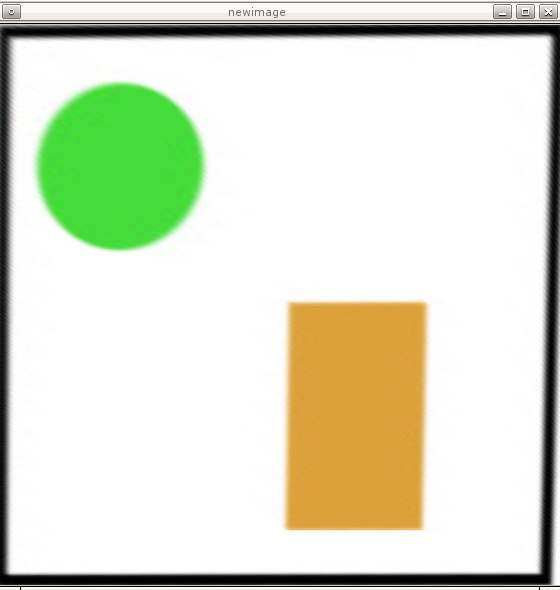
\includegraphics[width=0.7\textwidth]{figures/transformedImage.jpg}
	\caption{Rezultantna slika nakon transformacije}
	\label{fig:transformiranaSlika}
\end{figure}

Program završava pritiskom na tipku <ESC>

\section{Rezultati}
\label{sec:rezultati}